\hypertarget{ux9879ux76eeux53d1ux5c55ux901fux5ea6}{%
\subsubsection{项目发展速度}\label{ux9879ux76eeux53d1ux5c55ux901fux5ea6}}

问题:如何衡量组织的发展速度?

\hypertarget{ux63cfux8ff0}{%
\paragraph{描述}\label{ux63cfux8ff0}}

项目的发展速度是指议题数量、代码提交数量、更改请求数量和贡献者个数,作为``创新''的指标。

\hypertarget{ux76eeux6807}{%
\paragraph{目标}\label{ux76eeux6807}}

给开源项目办公室 (OSPO)
经理提供一种通过比较项目组合去衡量项目发展速度的方法。

OSPO 经理可以使用以下项目发展速度指标来:

\begin{itemize}
\tightlist
\item
  比较开源项目与内部项目的发展速度
\item
  比较项目组合中的项目发展速度
\item
  找出哪些项目外部贡献者的发展超出了内部贡献者(在筛选内部贡献者与外部贡献者时)
\item
  找出值得投入的有前途的领域
\item
  找出未来几年可能成功的领域
\end{itemize}

\href{https://www.cncf.io/blog/2017/06/05/30-highest-velocity-open-source-projects}{参见示例}

\hypertarget{ux5b9eux73b0}{%
\paragraph{实现}\label{ux5b9eux73b0}}

基本指标包括:

\begin{itemize}
\tightlist
\item
  \href{https://github.com/chaoss/wg-evolution/blob/master/metrics/Issues_Closed.md}{关闭的问题个数}
\item
  \href{https://github.com/chaoss/wg-evolution/blob/master/metrics/Reviews.md}{评论个数}
\item
  \href{https://github.com/chaoss/wg-evolution/blob/master/metrics/Code_Changes.md}{修改代码的人数}
\item
  \href{https://github.com/chaoss/wg-risk/blob/master/metrics/Committers.md}{代码提交人数}
\end{itemize}

\hypertarget{ux7b5bux9009ux6761ux4ef6}{%
\subparagraph{筛选条件}\label{ux7b5bux9009ux6761ux4ef6}}

\begin{itemize}
\tightlist
\item
  内部与外部贡献者
\item
  项目来源(例如,内部仓库、开源仓库和竞争对手的开源仓库)
\item
  时间
\end{itemize}

\hypertarget{ux53efux89c6ux5316ux6548ux679c}{%
\subparagraph{可视化效果}\label{ux53efux89c6ux5316ux6548ux679c}}

\begin{itemize}
\tightlist
\item
  X 轴:代码提交的总次数的对数
\item
  Y 轴:提交问题总个数和评论总个数之和的对数。
\item
  点大小:代码提交人数
\item
  点为某个项目
\end{itemize}

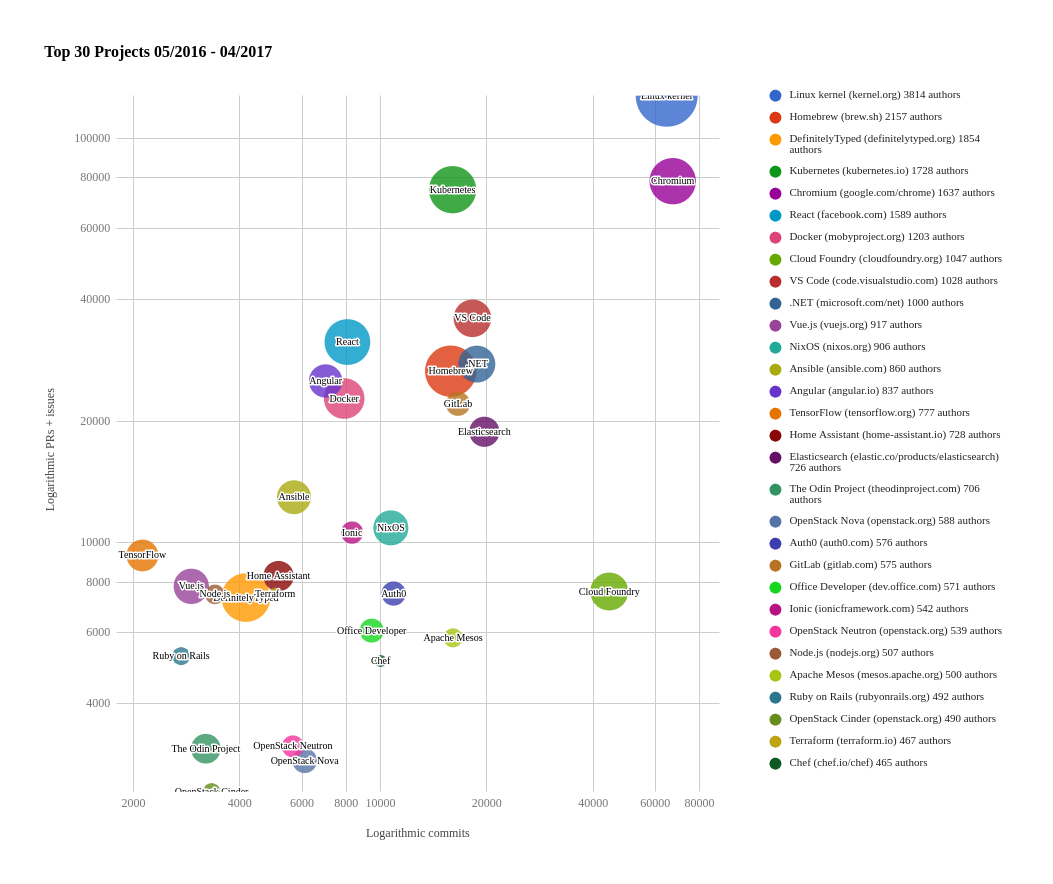
\includegraphics{images/project-velocity_visualization.png}

\href{https://www.cncf.io/blog/2017/06/05/30-highest-velocity-open-source-projects/}{来自
CNCF}

\hypertarget{ux63d0ux4f9bux6307ux6807ux7684ux5de5ux5177}{%
\subparagraph{提供指标的工具}\label{ux63d0ux4f9bux6307ux6807ux7684ux5de5ux5177}}

\begin{itemize}
\tightlist
\item
  CNCF -
  \href{https://github.com/cncf/velocity}{https://github.com/cncf/velocity}
\end{itemize}

\hypertarget{ux53c2ux8003ux8d44ux6599}{%
\paragraph{参考资料}\label{ux53c2ux8003ux8d44ux6599}}

\begin{itemize}
\tightlist
\item
  \href{https://www.threefivetwo.com/blog/can-open-source-innovation-work-in-the-enterprise}{开源创新能在企业中发挥作用吗?}
\item
  \href{https://www.nearform.com/blog/want-a-high-performing-culture-make-way-for-open-innovation}{高绩效文化的开放式创新}
\item
  \href{https://www.cio.com/article/3213146/open-source-is-powering-the-digital-enterprise.html}{数字企业的开源}
\item
  \href{https://www.cncf.io/blog/2017/06/05/30-highest-velocity-open-source-projects}{发展最快的开源项目}
\end{itemize}
